%!TEX root = /Users/Abj/git/MiL/report/report.tex
\part{Summary}

\section{About}
Musik i Lejet is a festival planned and executed by a group of volunteer arrangers. Over the last couple of years the festival has grown, and so has the workload and number of arrangers. In the current organizational setup, work domains are delegated to groups of arrangers. The groups must collaborate and coordinate their work, in areas where dependencies exist between them. If a task delegated to some group exceeds it deadline, it may cause a domino effect of postponing dependent tasks of other groups, thus affecting the entire organization. As the whole planning phase has a ultimo deadline each year, the festival itself, delayed tasks constitute a risk for the festival. The business case presented in the following aims to present an answer to the question:
\\
\begin{center}
\pbox{0.8\textwidth}{\textbf{How can the deadlines missed by team leaders, agreed upon at team leader meetings, be reduced by xx percentage?}}
\end{center}


\section{List of activities}
The following is a list of different activities we have conducted, consisting of interviews with and observations of the members of Mil.
\begin{center}
\begin{table}[H]
    \begin{tabular}{|p{3cm}|p{3cm}|p{3cm}|p{6cm}|}
    \hline
    \textbf{Date} & \textbf{Type of activity} & \textbf{Participants} & \textbf{Comments} \\ \hline
    29 - 09 - 13 & (informal) Interview & MiL: Andreas, ITU: All & The workgroup presented the scope(?) of the course and got an initial idea of the organization and the role that Andreas have in MiL.  \\ \hline
    31 - 10 - 13 & (formal) Interview & MiL: Christian og Stakkeman, ITU: Daniel, Jacob, Sune &  .......  \\ \hline
    17 - 11 - 13 & Observations & MiL: Board and Arrangers, ITU: Anders, Daniel, Jacob & Combined workshop and general assembly. \\ \hline
    20 - 11 - 13 & (formal) Interview & MiL: Andreas, ITU: Jacob, Jakob, Sune & .... \\ \hline
    21 - 11 - 13 & (formal) Interview & MiL: Stine, ITU: Jakob, Sune & .... \\ \hline
    \end{tabular}
\end{table}
\end{center}

\section{Figure of organization}
\label{sec:organisation}
This is a section of an organisational chart outlining the structure of Mil, made in collaboration with the board. The whole chart can be found in appendix XX: \\
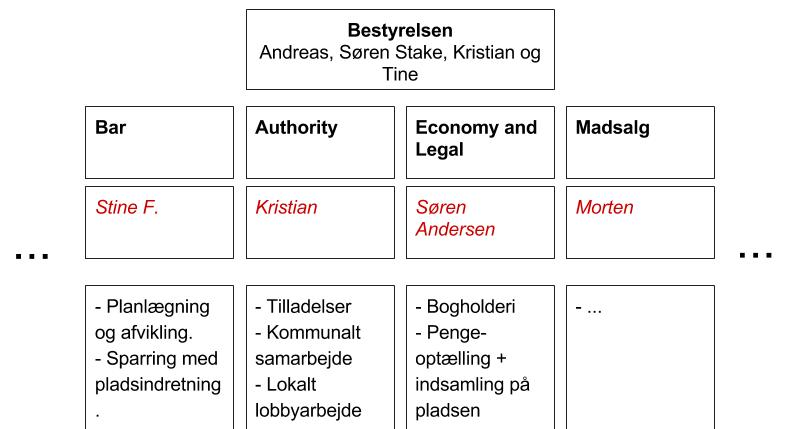
\includegraphics[scale=0.5]{Pictures/MIL_Organisational_chart_Cutout.jpg}
\section{Business and IT scope}
In this investigation we will focus on the managing part and more specific the arranger teams and team leaders of Musik I lejet. We will also look at how the internal communication is done, how information is shared between all members and what work processes are in play when planning the festival. \\
Most of the communication is done at Musik i Lejet's Podio site and therefore we will direct our attention and observations towards that platform. This is also the main IT-system used in the planning phase of the festival, when this is done, and as such this is where our focus on IT will be placed.
